%% Leakage-Controlled Evaluation Protocol --- Discover Internet of Things (Springer Nature)
%% Single self-contained manuscript file (sn-jnl class).
\documentclass[pdflatex,sn-mathphys-num]{sn-jnl}

\usepackage{graphicx}
\usepackage{multirow}
\usepackage{amsmath,amssymb,amsfonts}
\usepackage{amsthm}
\usepackage{mathrsfs}
\usepackage[title]{appendix}
\usepackage{xcolor}
\usepackage{textcomp}
\usepackage{booktabs}
\usepackage{algorithm}
\usepackage{algorithmicx}
\usepackage{algpseudocode}

\theoremstyle{thmstyleone}
\newtheorem{theorem}{Theorem}
\newtheorem{proposition}[theorem]{Proposition}
\theoremstyle{thmstyletwo}
\newtheorem{remark}{Remark}
\theoremstyle{thmstylethree}
\newtheorem{definition}{Definition}

\raggedbottom

\begin{document}

\title[A Leakage-Controlled Evaluation Protocol for DP Federated IoT Anomaly Detection]{A Leakage-Controlled Evaluation Protocol for Data Selection in Differentially Private Federated Anomaly Detection for Industrial IoT}

% ORCIDs (entered in submission system): Gaur 0000-0002-9570-4291;
% Raja 0000-0002-3663-1184; Rathore 0000-0002-4917-1500.
\author[1]{\fnm{Rishiraj Singh} \sur{Gaur}}\email{rishiraj.231051014@muj.manipal.edu}
\author[1]{\fnm{Linesh} \sur{Raja}}\email{linesh.raja@jaipur.manipal.edu}
\author*[2]{\fnm{Pramod Singh} \sur{Rathore}}\email{pramod.rathore@jaipur.manipal.edu}
\affil[1]{\orgdiv{Department of Computer Applications}, \orgname{Manipal University Jaipur}, \orgaddress{\city{Jaipur}, \country{India}}}
\affil[2]{\orgdiv{Department of Computer and Communication Engineering}, \orgname{Manipal University Jaipur}, \orgaddress{\city{Jaipur}, \country{India}}}

\abstract{Evaluating data selection under differential privacy (DP) is prone to methodological errors that can be mistaken for genuine effects. We contribute a
\emph{leakage-controlled evaluation protocol} for DP federated Industrial IoT (IIoT)
anomaly detection and demonstrate it against two failure modes of a standard pipeline. The first concerns utility: fitting the sample-selection gate on private,
anomaly-laden data and training the detector on the contaminated result produces a large deduplication ``gain'' ($+0.05$ to $+0.16$ F1 on the SWaT testbed) that
vanishes once the gate uses public normal-only data. The second concerns privacy: a
membership-inference attack that splits a client's stream into a contiguous first half
(``members'') and second half (``non-members'') reports AUC up to $0.73$ on SWaT (an apparent privacy leak), but this confounds membership with the
process's temporal drift; under a correctly randomized, seeded split the AUC collapses
to chance ($\approx0.50$, bootstrap $95\%$ CI including $0.5$) for both weak and strong
attacks. The protocol's requirements (public-only selection statistics, normal-only
detector training, accounted selection privacy, and randomized membership splits)
remove both artifacts. Under the leakage-controlled protocol the findings are consistent and mutually reinforcing: no learned selection rule beats uniform random subsampling or
full data across three datasets (one a saturation control), four budgets, and three
detector families; and no membership leakage is detectable on either testbed under the
attacks we run, contrary to what the confounded split suggested. The protocol and open code
help practitioners measure DP-IIoT privacy and utility without these confounds, rather than reporting
effects that do not exist.}

\keywords{Federated learning, Differential privacy, Anomaly detection,
Industrial IoT, Data deduplication, Membership inference, Reproducibility}

\maketitle

%%-----------------------------------------------------------------------------
\section{Introduction}\label{sec:intro}

Industrial IoT (IIoT) deployments such as water treatment plants and chemical
reactors stream readings from many sensors to edge nodes that must detect
anomalies without centralising sensitive operational data. Federated learning
(FL)~\cite{mcmahan2017communication} trains a shared detector from local updates,
and differential privacy (DP)~\cite{abadi2016deep} bounds what those updates
reveal. Because high-rate sensors produce many \emph{near-duplicate} readings,
a natural idea is to remove this redundancy \emph{before} DP training: fewer,
non-redundant samples mean fewer gradient steps, and, under a fixed end-to-end
$(\varepsilon,\delta)$ budget, less injected DP noise. Several recent trends make
the idea attractive, from semantic deduplication for large-scale
training~\cite{lee2022dedup,abbas2023semdedup} to coreset and data-pruning
methods~\cite{marion2023scaling}.

Whether or not one pursues this particular idea, it exposes a broader problem:
\emph{evaluating data selection under DP is susceptible to errors that can appear as valid results}, on both the utility and the privacy axis. On the utility side, the statistics
used to choose samples can leak private information into the pipeline, and an anomaly
detector trained carelessly can reward selection for the wrong reason. On the privacy
side, the way the data is split to test for membership leakage can confound membership
with the natural drift of an industrial process. Either error produces a false but confident-looking conclusion---the kind of evaluation leakage that a recent
survey found in $294$ papers across $17$ scientific fields~\cite{kapoor2023leakage}.

This paper offers a \emph{leakage-controlled evaluation protocol} for data selection in
DP federated IIoT anomaly detection and demonstrates it against two such failure modes on real
industrial control-system (ICS) data. The utility failure mode: a protocol-violating pipeline produces a large but spurious deduplication gain that the protocol
erases, after which no selection rule we tried improves the privacy--utility tradeoff,
consistent with recent theory on record suppression~\cite{stoddard2026suppress}. The privacy failure mode: a membership-inference test that uses a contiguous temporal split
reports AUC up to $0.73$ on SWaT (an apparent leak), but with a correctly randomized,
seeded split the signal collapses to chance for both weak and strong attacks, so the conclusion is that no leakage is detectable here. Both failure modes are easy to overlook and, once removed, the picture is consistent: selection does not help, and we
find no evidence that the DP guarantee is failing.

\paragraph{Contributions.}
\begin{enumerate}
  \item \textbf{A leakage-controlled evaluation protocol for data selection under DP
    (\S\ref{sec:setup}).} Four requirements that together prevent a class of
    measurement errors: (i) compute all selection statistics on \emph{public}
    data only; (ii) train the reconstruction detector on \emph{normal-only} data;
    (iii) account for the privacy cost of any data-dependent
    selection~\cite{nguyen2025coreset}; and (iv) evaluate membership leakage with a
    \emph{randomized, seeded} member/non-member split. Each is individually known; we
    show that together, in this setting, omitting any one produces a spurious result.
  \item \textbf{A utility artifact (\S\ref{sec:res-artifact}).} A natural but
    protocol-violating pipeline produces a large apparent deduplication advantage on
    SWaT---from fitting the selection gate on \emph{private, anomaly-laden} data and
    training the detector on \emph{contaminated} data. Under the protocol the
    advantage vanishes. We release both pipelines so the false positive is
    independently reproducible.
  \item \textbf{A privacy artifact, and no detectable leakage under a randomized split
    (\S\ref{sec:res-privacy}).} A membership-inference test with a contiguous temporal
    member/non-member split reports AUC up to $0.73$ on SWaT, but this confounds
    membership with process drift: even a weak attack shows it, and a randomized split
    returns chance ($\approx0.50$, CI including $0.5$) for both weak and strong
    attacks over $5$ seeds. Under the randomized split we find no membership leakage
    detectable by the attacks we run---consistent with the DP guarantee, though not a
    proof of protection against an unbounded adversary.
  \item \textbf{No learned selection rule helps, on the datasets evaluated
    (\S\ref{sec:res-selection}, \S\ref{sec:res-strong}).} Learned temporal
    deduplication and a diversity coreset never beat uniform random subsampling or
    full data, across datasets, budgets, three detector families (reconstruction
    autoencoder, Isolation Forest, One-Class SVM), and centralised and federated
    settings, consistent with a recent suppression
    theorem~\cite{stoddard2026suppress,nguyen2025coreset,ayle2023bagging}.
\end{enumerate}
We additionally provide runtime measurements, strong non-private reference
detectors, and open code.

\begin{figure}[t]
\centering
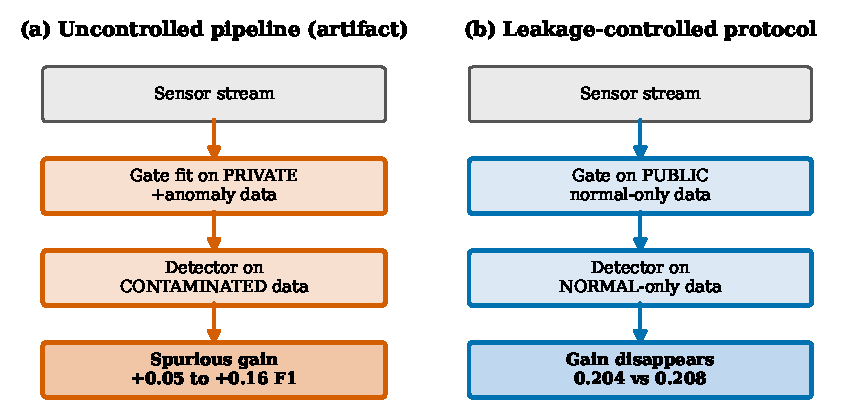
\includegraphics[width=\linewidth]{figs/fig_schematic}
\caption{The two pipelines (uncontrolled in orange, leakage-controlled in blue). (a) The uncontrolled implementation fits the selection gate on private, anomaly-laden data and trains the
detector on the contaminated result, producing a spurious $+0.05$ to $+0.16$ F1
``gain''. (b) The leakage-controlled protocol fits the gate on public normal-only data
and trains on normal-only data; the gain disappears ($0.204$ vs.\ $0.208$).}\label{fig:schematic}
\end{figure}

\section{Background and Related Work}\label{sec:related}

\paragraph{DP-SGD and federated learning.} DP-SGD~\cite{abadi2016deep} clips
per-sample gradients and adds Gaussian noise; privacy is tracked with the RDP
accountant~\cite{mironov2017renyi}. We use record-level DP and calibrate the noise
multiplier to the \emph{end-to-end} budget over all rounds. Federated averaging
aggregates client updates~\cite{mcmahan2017communication,li2020federated}.

\paragraph{FL anomaly detection for IIoT.} Reconstruction autoencoders are the
workhorse detector for sensor streams~\cite{wang2021industrial,aslam2025optimized}, and a
growing line of FL work applies them to industrial and network anomaly
detection~\cite{liu2020fl,rey2022federated,mothukuri2021anomaly}. Privacy-preserving FL
for industrial and IoT intrusion and anomaly detection is now a busy
subfield~\cite{alqazzaz2026secufl,zhu2025cutting,selvam2025federated,sharma2025privacy,
khraisat2025federated,karunamurthy2025optimal,laghari2025novel,liang2025optimization},
spanning graph- and deep-network detectors for IoT
anomalies~\cite{altfaily2025graph,sathyabama2025enhancing}, on-device detection at the
edge~\cite{arciniegas2025iot}, and federated designs for securing IoT
data~\cite{wankhede2025federated}. A subset couples the detector with a formal privacy
mechanism such as DP, or with federated defenses for cyber-physical
systems~\cite{ramana2025trust,deng2025anomaly,chen2024differential}. These works report
positive results, but they evaluate without a DP budget, or with privacy bolted on after
training rather than treated as a constraint that interacts with every preprocessing
choice. That gap matters here: a
reconstruction detector only works when trained on \emph{normal} data, so any
selection or labelling step that lets anomalies leak into the training set degrades the detector. We show in \S\ref{sec:res-artifact} that this exact error, combined with private-data leakage into the selection statistics, is enough to
produce a spurious gain.

\paragraph{Deduplication, coresets and DP.} Semantic
deduplication~\cite{abbas2023semdedup} and data pruning~\cite{marion2023scaling}
reduce training sets for large models, typically choosing thresholds to hit a
target size rather than on principled grounds. In the DP setting, however, recent
analyses show that removing records does not reliably help, and often hurts, the
privacy--utility tradeoff. Most directly, Miranda-Pascual et
al.~\cite{stoddard2026suppress} show, in a recent preprint, that a deterministic
suppression map composes with DP so that its \emph{sensitivity multiplies} the privacy
cost (their Theorem~5.1): at \emph{equal} privacy, omitting records cannot improve the
tradeoff for the canonical mechanisms. This is the formal reason the intuition
``fewer samples $\Rightarrow$ less noise $\Rightarrow$ better utility'' fails---the
saved noise is paid back as increased sensitivity of the selection step. Relatedly,
uniform random subsampling is a strong baseline in the high-compression
regime~\cite{ayle2023bagging}, and data-dependent selection itself consumes privacy
budget~\cite{nguyen2025coreset}. We treat~\cite{stoddard2026suppress} as an
interpretive lens rather than a validated prediction: it is a recent preprint, and a
reader who doubts its generality can set it aside without affecting our empirical
claims, which rest on the measurements that follow. Its role is to explain
\emph{why} those measurements come out as they do.

\paragraph{Membership inference.} Membership-inference attacks quantify privacy
leakage~\cite{shokri2017membership}; calibrated likelihood-ratio attacks such as
LiRA~\cite{carlini2022membership} are the standard strong baseline, and in federated
training the attacker can be stronger still~\cite{nasr2019comprehensive}. Less
discussed is that the \emph{evaluation design} can dominate the result: how the data
is partitioned into members and non-members determines what the AUC measures. If the
split correlates with any non-membership signal (temporal order being the obvious one
for a drifting process), the attack scores that signal instead of membership.
\S\ref{sec:res-privacy} shows our own pipeline exhibits exactly this failure mode, and that
the apparent leakage disappears once the split is randomized.

\section{Leakage-Controlled Setup}\label{sec:setup}

\paragraph{Detector and selection.} The detector is a small reconstruction
autoencoder; the anomaly score is per-sample reconstruction error thresholded at a
percentile. Crucially, it is trained on \emph{normal-operation data only}. When a
subset is used, it is chosen by one of: uniform \emph{random} subsampling;
\emph{temporal} deduplication (a sequential rule that keeps a sample only when its
learned-embedding cosine similarity to the last kept sample falls below a threshold
set at the median of the observed consecutive-similarity distribution, i.e.\ a
keep-quantile of $0.5$, computed on public data); or a \emph{diversity coreset}
(greedy farthest-point sampling in the same embedding, which approximates the
$k$-centre objective). The embedding for both learned rules comes from a single shared
encoder (an MLP with hidden layers of $128$ and $64$ units and an output dimension of
$16$ on SKAB and $32$ on SWaT and TEP, trained on public normal data with a
temporal-proximity contrastive loss), so the temporal and diversity rules differ only
in their selection criterion, not their representation. The encoder is trained with a
triplet margin loss ($\ell_2$, margin $0.5$) in which the anchor and positive are
temporal neighbours within $\pm$window and the negative is a uniformly sampled normal
record; embeddings are $\ell_2$-normalised so similarity is cosine. The reconstruction
detector is a symmetric autoencoder whose decoder mirrors the encoder
(bottleneck$\to$$h_2$$\to$$h_1$$\to$input, ReLU activations). The
temporal rule fixes the budget; random and diversity are then matched to that same
size for a fair comparison. In practice this retains about $37\%$ of the normal data
on SKAB and $49\%$ on SWaT. Where we partition data across clients non-IID, we use a
Dirichlet split with concentration $\alpha{=}0.5$.

\paragraph{Selection statistics use public data only.} Any statistic used to
select or preserve samples (e.g.\ the $3\sigma$ exceedance gate, computed
\emph{per feature} as $\max_j |x_j-\mu_j|/\sigma_j > \gamma$) is estimated only on
a public normal-operation reference set, never on private or anomaly-labelled
client data. Accounting for the data-dependent selection map explicitly, its privacy cost
must be accounted alongside training ($\varepsilon=\varepsilon_{\text{sel}}+
\varepsilon_{\text{train}}$)~\cite{nguyen2025coreset}; using public-only statistics
makes $\varepsilon_{\text{sel}}=0$.

\paragraph{Membership-inference evaluation.} To test whether the trained detector
leaks membership, members and non-members must be drawn by a \emph{randomized} split
of the normal data, not by any partition correlated with non-membership signal. On a
drifting industrial process a contiguous temporal split (first half members, second
half non-members) is such a confound; we use a uniformly random member assignment and
average over $5$ seeds, reporting a bootstrap $95\%$ confidence interval on the AUC.
We verify this matters in \S\ref{sec:res-privacy}.

\paragraph{Datasets.} \textbf{SKAB}~\cite{katser2020skab} (water-pump testbed,
$d{=}8$, $28.3\%$ anomaly), \textbf{SWaT}~\cite{mathur2016swat,goh2016swat}
(Secure Water Treatment, July~2019 collection, $d{=}44$, $13.2\%$ attack; labels
reconstructed from the six documented attack windows), and \textbf{TEP}
(Tennessee Eastman process~\cite{downs1993tep,rieth2017tep}, $d{=}52$: $41$
measurement and $11$ manipulated variables, $35\%$ fault) span no-to-high
redundancy. Machine-learning attack detection on public ICS testbeds of this kind is
well established~\cite{mubarak2022industrial}. We use $K{=}5$ clients, $R{=}15$ rounds,
end-to-end $\varepsilon\in\{0.5,1,2,4\}$, $\delta{=}10^{-5}$.

\section{Results}\label{sec:results}

\subsection{Apparent utility gains are preprocessing artifacts}\label{sec:res-artifact}
A natural first implementation that (i) fit the $3\sigma$ preservation gate on the
full training data (including anomalies) and (ii) trained the detector on the
resulting anomaly-enriched set produced a large apparent SWaT advantage for
deduplication---of order $+0.05$ to $+0.16$ F1 over same-budget DP-FL across
budgets (\texttt{paper\_results.json}), the kind of result that would headline a
positive paper. When the gate is instead fit on public normal-only data (both
leakage-controlled and statistically correct, since anomalies should not define the
``normal'' envelope) the advantage disappears: on SWaT, averaged over budgets,
partitions and $10$ seeds, training with deduplication reaches F1 $0.204$ versus
$0.208$ without it (\texttt{honest\_rerun.json}). We do not lean on that small gap,
which is itself within noise. Table~\ref{tab:artifact} shows the per-cell picture:
once the gate is fit on public normal-only data, the deduplication and
no-deduplication columns overlap within one standard deviation in \emph{every} cell,
across both IID and non-IID (Dirichlet) partitions. The large headline advantage is
simply gone; it was an artifact of the gate and detector seeing data they should not
have, not a property of deduplication. This pipeline is representative of common
practice rather than a straw man: recent federated IoT intrusion-detection studies
report strong results without calibrating an end-to-end DP budget or an evaluation
designed to rule out the leakage studied here
(e.g.,~\cite{khraisat2025federated,karunamurthy2025optimal}). A factorial ablation (Supplement, including a
table that decomposes the $2\times2$ of the two utility rules) shows that fixing
\emph{either} rule independently removes most of the gain, and that normal-only
training is the load-bearing requirement: once it holds, the gate-reference choice has
no further effect on utility.

\begin{table}[t]
\centering
\caption{Artifact audit (federated, corrected public-normal gate). SWaT F1
(mean$\pm$std, $10$ seeds); after the fix the deduplication and no-deduplication
columns overlap within one standard deviation in every cell. Source:
\texttt{honest\_rerun.json}}\label{tab:artifact}
\setlength{\tabcolsep}{3.5pt}
\begin{tabular}{@{}llcccc@{}}
\toprule
Partition & Method & $\varepsilon{=}0.5$ & $\varepsilon{=}1$ & $\varepsilon{=}2$ & $\varepsilon{=}4$ \\
\midrule
\multirow{2}{*}{IID} & no-dedup & 0.221$\pm$0.010 & 0.219$\pm$0.008 & 0.220$\pm$0.033 & 0.185$\pm$0.025 \\
 & dedup & 0.229$\pm$0.016 & 0.206$\pm$0.018 & 0.210$\pm$0.014 & 0.180$\pm$0.023 \\
\midrule
\multirow{2}{*}{Dir.} & no-dedup & 0.231$\pm$0.044 & 0.219$\pm$0.060 & 0.174$\pm$0.021 & 0.198$\pm$0.034 \\
 & dedup & 0.218$\pm$0.019 & 0.211$\pm$0.044 & 0.196$\pm$0.044 & 0.182$\pm$0.037 \\
\botrule
\end{tabular}
\end{table}

\subsection{No learned selection rule beats random or full}\label{sec:res-selection}
To isolate the effect of \emph{which} samples are selected from the effects of
federation, this comparison uses centralised DP training; the artifact audit in
\S\ref{sec:res-artifact} is already in the full federated setting.
Table~\ref{tab:char} compares full normal data against three matched-size
selection rules under DP, with standard deviations over $10$ seeds. On \textbf{SKAB}
the four conditions are equal within seed noise (cross-mode spread
$0.001$--$0.005$, smaller than the per-cell std): reduction is neutral and the
choice of rule is irrelevant. On \textbf{SWaT} the seed-to-seed std is large (up to
$\pm0.049$), and the cross-mode differences sit \emph{within} these bands: the
apparent crossings (full best at $\varepsilon{=}0.5$, random best at
$\varepsilon{=}2$) are not statistically distinguishable from noise, so we do not
read them as a real ``random helps'' effect. What the data do support is the absence
of any \emph{learned}-rule advantage: temporal deduplication
and the diversity coreset never exceed random or full beyond one standard deviation,
in any dataset or budget. On \textbf{TEP} ($\rho\approx1$) the detector saturates at
the percentile threshold and all conditions are identical ($0.444$): a saturation
control (\texttt{characterization.json}).

\paragraph{Federated setting.} The centralised setting isolates the
selection effect, but the system is federated, so we re-ran the full four-arm
comparison with FedAvg over $K{=}5$ contiguous client partitions (the regime where
local deduplication might plausibly interact with aggregation). Table~\ref{tab:fedarms}
reports it. The result matches the centralised setting: no learned rule separates from random; pooling
the federated runs ($n{=}40$ paired comparisons each), temporal deduplication differs
from random by $-0.002$ F1 (Wilcoxon $p=0.57$) and the diversity coreset by $+0.001$
($p=0.83$); the best-scoring method alternates arbitrarily across cells
(\texttt{fed\_allarms.json}).
This matters because an earlier federated sweep \emph{without} a random arm had shown
deduplication beating \emph{full} data in most cells, a result that, read alone,
looks like a win for deduplication. The all-arms comparison shows why it is not:
random subsampling captures the same effect, so the gain belongs to using fewer
samples under DP, not to the learned rule. The null holds in the titular federated
setting, not just centrally.

\paragraph{Federation scale.} A natural worry is that $K{=}5$ is too small for the
aggregation dynamics that might make local deduplication matter. We therefore repeat
the all-arms comparison at $K{=}10$ and $K{=}20$ contiguous clients
(Table~\ref{tab:kabl}, \texttt{fed\_kablation.json}, $5$ seeds). The conclusion is
unchanged at both scales: pooled over the $80$ paired runs, the learned rules differ
from random by $-0.001$ F1 and from full by $-0.007$ F1. On SKAB the four arms sit
within one standard deviation; on SWaT full data is the best arm and no learned rule
beats it. Growing the fleet does not create a deduplication advantage. We are candid
about one boundary: under a far more heterogeneous Dirichlet($\alpha{=}0.1$) split
(\texttt{fed\_dirichlet01.json}), the per-client data becomes so small and skewed that
every arm turns highly variable (std up to $\pm0.11$ on SWaT), and the pooled
learned-vs-random difference is $+0.015\pm0.034$, positive but swamped by that
variance, with individual cells swinging both ways. We do not read this as a learned
advantage; rather, at this extreme heterogeneity our five-seed experiment simply lacks
the power for a clean statement, and we report it as such.

\begin{table}[t]
\centering
\caption{Federation scale ($K{=}10, 20$ contiguous clients). F1 (mean$\pm$std, $5$
seeds). The null persists as the fleet grows: no learned rule beats random or full.
Source: \texttt{fed\_kablation.json}}\label{tab:kabl}
\setlength{\tabcolsep}{3.5pt}
\begin{tabular}{@{}lllcccc@{}}
\toprule
Data & $K$ & $\varepsilon$ & full & random & temporal & diversity \\
\midrule
\multirow{4}{*}{SKAB} & \multirow{2}{*}{10} & 0.5 & 0.190$\pm$0.006 & 0.197$\pm$0.007 & 0.197$\pm$0.005 & 0.198$\pm$0.005 \\
 & & 2.0 & 0.181$\pm$0.004 & 0.194$\pm$0.007 & 0.190$\pm$0.004 & 0.194$\pm$0.009 \\
 & \multirow{2}{*}{20} & 0.5 & 0.198$\pm$0.005 & 0.193$\pm$0.002 & 0.194$\pm$0.002 & 0.193$\pm$0.001 \\
 & & 2.0 & 0.191$\pm$0.003 & 0.195$\pm$0.004 & 0.201$\pm$0.005 & 0.197$\pm$0.008 \\
\midrule
\multirow{4}{*}{SWaT} & \multirow{2}{*}{10} & 0.5 & 0.246$\pm$0.011 & 0.226$\pm$0.027 & 0.226$\pm$0.007 & 0.241$\pm$0.031 \\
 & & 2.0 & 0.293$\pm$0.013 & 0.255$\pm$0.020 & 0.265$\pm$0.007 & 0.236$\pm$0.025 \\
 & \multirow{2}{*}{20} & 0.5 & 0.221$\pm$0.011 & 0.223$\pm$0.020 & 0.208$\pm$0.017 & 0.216$\pm$0.012 \\
 & & 2.0 & 0.235$\pm$0.011 & 0.225$\pm$0.021 & 0.222$\pm$0.017 & 0.222$\pm$0.006 \\
\botrule
\end{tabular}
\end{table}

\begin{table}[t]
\centering
\caption{Selection has no advantage. F1 (mean$\pm$std, $10$ seeds, centralised DP,
normal-only training) for full data vs.\ matched-size random / temporal-dedup /
diversity-coreset selection. No learned rule beats random or full beyond noise.
Source: \texttt{characterization.json}}\label{tab:char}
\setlength{\tabcolsep}{4pt}
\begin{tabular}{@{}llcccc@{}}
\toprule
Dataset & $\varepsilon$ & full & random & temporal & diversity \\
\midrule
\multirow{4}{*}{SKAB} & 0.5 & 0.210$\pm$0.004 & 0.207$\pm$0.002 & 0.207$\pm$0.002 & 0.207$\pm$0.004 \\
 & 1.0 & 0.213$\pm$0.012 & 0.208$\pm$0.004 & 0.209$\pm$0.004 & 0.208$\pm$0.004 \\
 & 2.0 & 0.214$\pm$0.013 & 0.210$\pm$0.006 & 0.212$\pm$0.007 & 0.209$\pm$0.009 \\
 & 4.0 & 0.214$\pm$0.013 & 0.211$\pm$0.009 & 0.211$\pm$0.011 & 0.212$\pm$0.010 \\
\midrule
\multirow{4}{*}{SWaT} & 0.5 & 0.366$\pm$0.017 & 0.329$\pm$0.008 & 0.317$\pm$0.002 & 0.315$\pm$0.003 \\
 & 1.0 & 0.325$\pm$0.049 & 0.350$\pm$0.016 & 0.324$\pm$0.004 & 0.321$\pm$0.004 \\
 & 2.0 & 0.321$\pm$0.042 & 0.361$\pm$0.021 & 0.326$\pm$0.006 & 0.325$\pm$0.005 \\
 & 4.0 & 0.325$\pm$0.037 & 0.337$\pm$0.040 & 0.303$\pm$0.024 & 0.304$\pm$0.029 \\
\midrule
TEP & 0.5--4 & 0.444$\pm$0.000 & 0.444$\pm$0.000 & 0.444$\pm$0.000 & 0.444$\pm$0.000 \\
\botrule
\end{tabular}
\end{table}

\begin{table}[t]
\centering
\caption{Federated all-arms comparison (FedAvg, $K{=}5$ contiguous clients,
end-to-end DP). F1 (mean$\pm$std, $5$ seeds). No learned rule (temporal, diversity)
beats random or full; the best method alternates across cells. Source:
\texttt{fed\_allarms.json}}\label{tab:fedarms}
\setlength{\tabcolsep}{4pt}
\begin{tabular}{@{}llcccc@{}}
\toprule
Dataset & $\varepsilon$ & full & random & temporal & diversity \\
\midrule
\multirow{2}{*}{SKAB} & 0.5 & 0.182$\pm$0.003 & 0.185$\pm$0.002 & 0.191$\pm$0.006 & 0.188$\pm$0.002 \\
 & 2.0 & 0.178$\pm$0.010 & 0.189$\pm$0.004 & 0.186$\pm$0.002 & 0.187$\pm$0.005 \\
\midrule
\multirow{2}{*}{SWaT} & 0.5 & 0.289$\pm$0.005 & 0.260$\pm$0.020 & 0.262$\pm$0.015 & 0.264$\pm$0.008 \\
 & 2.0 & 0.281$\pm$0.053 & 0.303$\pm$0.009 & 0.298$\pm$0.011 & 0.296$\pm$0.006 \\
\botrule
\end{tabular}
\end{table}

\begin{figure}[t]
\centering
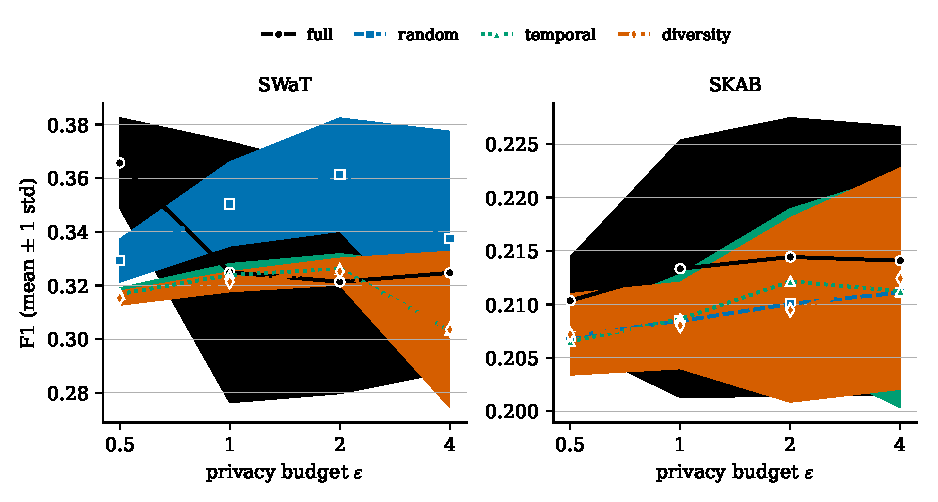
\includegraphics[width=\linewidth]{figs/fig_frontier}
\caption{Selection-invariance frontier: F1 versus privacy budget for full data and
the three matched-size selection rules, with $\pm1$ standard-deviation bands over $10$
seeds (\texttt{characterization.json}). The bands overlap throughout; no learned rule
(temporal, diversity) separates from random or full at any budget.}\label{fig:frontier}
\end{figure}

\paragraph{Statistical analysis.} We test the learned rules against random, reporting
a Wilcoxon signed-rank test, a two-one-sided-test (TOST) equivalence check, and Cohen's
$d_z$ over $10$ seeds (\texttt{stats\_tests.json}). Because pooling across budgets
mixes runs with different noise multipliers, the per-budget tests ($n{=}10$ each) are
the primary statistic and the pooled test ($n{=}40$) is secondary. The equivalence
margin for TOST is $\pm0.02$ F1, pre-specified as the smallest difference we would
treat as practically meaningful for these detectors; it lies below the typical
per-cell standard deviation ($0.02$--$0.05$), and for context the largest cross-mode
F1 gap we observe under DP is $0.050$ (SWaT at $\varepsilon{=}0.5$;
\texttt{characterization.json}). Per
budget, in no case does a learned rule exceed random by more than $0.002$ F1 on either
dataset. Pooled, on SKAB the learned rules are statistically \emph{equivalent} to
random (TOST $p<0.001$; Wilcoxon $p>0.63$; $|d_z|<0.18$), and on SWaT they are
significantly \emph{worse} than random (Wilcoxon $p<0.001$; mean $-0.027$ F1;
$d_z\approx-1.1$). In neither case is a learned rule better than the trivial baseline;
the only statistically reliable effect points against them. The direction is
consistent across all budgets, which we treat as the load-bearing evidence. We report
these tests as exploratory and apply no formal multiple-comparison correction; every
reliable effect points the same way, so a correction would not change the conclusion.

\subsection{Robustness to detector strength}\label{sec:res-strong}
The absence of an advantage might instead reflect a detector
operating near the random-score floor (F1 $\approx0.13$--$0.15$;
\S\ref{sec:res-context}), where no training subset could matter. We test this by
training the same reconstruction detector far longer (normal-only, $40$ epochs) and
repeating the selection comparison (Table~\ref{tab:strong}). We report two metrics.
Point-wise F1 is the appropriate one. Point-adjusted F1 is included only for comparability
with the strong-detector literature, which uses it widely; we flag that it inflates
scores: Kim et al.~\cite{kim2022rigorous} show even random scores reach high
point-adjusted F1, and Wu and Keogh~\cite{wu2021flawed} argue such benchmarks create
an illusion of progress; the broader metric landscape is surveyed
by~\cite{sorbo2024navigating}. We do not treat it as a measure of true detection
quality. The
selection conclusion is unchanged under both. Under point-wise F1 the learned rules
trail random by $0.036$--$0.098$ on SWaT; under point-adjusted F1, where every method
is pushed to $\approx0.65$, no rule separates from the others (spreads $<0.03$); on
SKAB all conditions are within one standard deviation
(\texttt{strong\_selection.json}). When the inflation-prone metric pushes all methods
to the same score and the point-wise metric still shows no learned advantage, selection
is not the lever---consistent with the recent (preprint) suppression result
of~\cite{stoddard2026suppress}. The null is a property of selection-under-DP, not of a
weak detector.

\paragraph{Limit of the high-signal evidence.} Under
DP, point-wise F1 stays modest because the noise caps it. To probe the floor-effect
objection at its strongest, we removed DP and trained the $40$-epoch detector to its
best point-wise score (\texttt{high\_signal\_selection.json}, $5$ seeds). On
SWaT it reaches F1 $0.430\pm0.026$, about three times the $0.13$ random-score floor
and on par with the non-private Isolation Forest ($0.39$) and One-Class SVM ($0.40$)
of \S\ref{sec:res-context}. At this level---where the detector demonstrably
works---the four arms stay within noise (full $0.430$, random $0.425$, temporal
$0.414$, diversity $0.436$; spread $0.022$, below the per-cell standard deviation),
and under light DP ($\varepsilon{=}8$) full data is best ($0.389$) while the learned
rules again fail to beat random. SKAB behaves the same way, with all four arms within
$0.013$ F1 at every setting (\texttt{high\_signal\_selection.json}). We are
deliberately explicit about what this does
\emph{not} establish: we could not push this reconstruction detector above point-wise
F1 $\approx0.45$ on these testbeds, so whether the null would persist in a genuinely
high-signal regime (point-wise F1 $>0.6$, which some sequence models report only under
point-adjustment) is beyond what our detector can demonstrate. We flag this as a real
limitation rather than claim the stronger result.

\begin{table}[t]
\centering
\caption{Longer-trained detector ($40$ epochs). F1 (mean$\pm$std, $10$ seeds,
DP). Point-wise is the appropriate metric; point-adjusted (PA) is inflation-prone and
shown for comparability only. No learned rule beats random or full under either.
Source:
\texttt{strong\_selection.json}}\label{tab:strong}
\setlength{\tabcolsep}{4pt}
\begin{tabular}{@{}llcccc@{}}
\toprule
 & $\varepsilon$ & full & random & temporal & diversity \\
\midrule
\multicolumn{6}{@{}l}{\emph{SWaT, point-adjusted F1}}\\
 & 0.5 & 0.651$\pm$0.010 & 0.657$\pm$0.005 & 0.648$\pm$0.001 & 0.647$\pm$0.001 \\
 & 2.0 & 0.648$\pm$0.007 & 0.649$\pm$0.013 & 0.624$\pm$0.007 & 0.626$\pm$0.010 \\
\multicolumn{6}{@{}l}{\emph{SWaT, point-wise F1}}\\
 & 0.5 & 0.335$\pm$0.036 & 0.357$\pm$0.018 & 0.321$\pm$0.004 & 0.319$\pm$0.003 \\
 & 2.0 & 0.321$\pm$0.028 & 0.324$\pm$0.049 & 0.226$\pm$0.030 & 0.236$\pm$0.039 \\
\multicolumn{6}{@{}l}{\emph{SKAB, point-adjusted F1}}\\
 & 0.5 & 0.700$\pm$0.026 & 0.768$\pm$0.007 & 0.762$\pm$0.021 & 0.756$\pm$0.026 \\
 & 2.0 & 0.696$\pm$0.029 & 0.693$\pm$0.030 & 0.697$\pm$0.024 & 0.696$\pm$0.024 \\
\multicolumn{6}{@{}l}{\emph{SKAB, point-wise F1}}\\
 & 0.5 & 0.212$\pm$0.010 & 0.208$\pm$0.002 & 0.210$\pm$0.002 & 0.209$\pm$0.003 \\
 & 2.0 & 0.216$\pm$0.010 & 0.214$\pm$0.011 & 0.216$\pm$0.010 & 0.216$\pm$0.012 \\
\botrule
\end{tabular}
\end{table}

\paragraph{Other detector families.} To confirm the null is not specific to the
reconstruction autoencoder, we repeated the four-arm
selection comparison with two detector families that are not gradient-trained, an
Isolation Forest and a One-Class SVM, on the same normal-only subsets
(\texttt{alt\_detector.json}). The verdict carries over: no learned rule beats random
or full. On SKAB the four conditions are within $0.002$--$0.011$ F1; on SWaT, where
reduction matters more, full data is best and the learned rules are \emph{worst}
(Isolation Forest full $0.393$ vs.\ temporal $0.286$, diversity $0.255$; One-Class
SVM full $0.405$ vs.\ both learned rules $0.374$). These detectors are non-private,
so this isolates a separate point from the DP analysis: the irrelevance of \emph{which}
samples are kept is a property of the selection problem, not an artifact of one model.

\subsection{Performance in context}\label{sec:res-context}
Absolute F1 is modest because anomaly detection on these testbeds is intrinsically
hard for a lightweight reconstruction detector. A non-private \emph{Isolation
Forest}~\cite{liu2008isolation} under the same protocol reaches only F1 $0.20$
(SKAB) and $0.33$ (SWaT) (\texttt{reference\_baselines.json}), and a trivial
random-score detector reaches $0.149$/$0.130$. The DP detectors operate in this
regime; the point of this study is the \emph{absence of a deduplication advantage},
not absolute state-of-the-art detection.

\subsection{A second artifact: membership leakage from the evaluation split}\label{sec:res-privacy}
Our second case study concerns privacy evaluation, where the same confound affects a strong attack as much as a weak one. A natural membership-inference setup labels the first
temporal half of a client's normal stream as \emph{members} (the detector's training
data) and the second half as \emph{non-members}. On a process that drifts over time,
this confounds membership with distribution shift: the detector has lower loss on the
first half because it is a different slice of the series, not because those points
were training members. Table~\ref{tab:mia} shows the consequence. Under this
contiguous split, even a weak loss-threshold attack reports AUC up to $0.73$ on SWaT,
and a calibrated LiRA attack~\cite{carlini2022membership} reports $0.73$ as
well---both of which read as ``DP leaks''. The reading is spurious. When the
member/non-member assignment is instead randomized and averaged over $5$ seeds, every
AUC collapses to chance: weak and LiRA both $\approx0.50$, with bootstrap $95\%$
confidence intervals that include $0.5$ at both budgets on both datasets
(\texttt{lira\_mia.json}; the contiguous split is \texttt{mia\_artifact.json}). The
apparent leakage was an artifact of the evaluation split, not a property of the model.
Note that attack strength is not the issue---the weak attack shows the inflation
too---so the fix is not ``use a stronger attack'' but ``use a correctly randomized,
seeded membership split.'' Under the randomized evaluation we find no membership leakage
detectable on either testbed. We state this precisely: it is evidence of no leakage
\emph{under the attacks we run, with $N{=}8$ non-private reference models}, not a proof
of protection against an unbounded or adaptive adversary; it is consistent with the DP
guarantee rather than a measurement of it.

\begin{table}[t]
\centering
\caption{Membership-inference AUC (mean$\pm$std, $5$ seeds; $0.5$ = chance). A contiguous (temporal) member/non-member split produces apparent leakage that
neither a weak nor a strong attack should be trusted to report; a randomized split
returns chance. Source: \texttt{mia\_artifact.json} (contiguous split), \texttt{lira\_mia.json} (randomized split)}\label{tab:mia}
\setlength{\tabcolsep}{4pt}
\begin{tabular}{@{}lcccc@{}}
\toprule
 & \multicolumn{2}{c}{contiguous split} & \multicolumn{2}{c}{randomized split} \\
\cmidrule(lr){2-3}\cmidrule(lr){4-5}
Setting & weak & LiRA & weak & LiRA \\
\midrule
SKAB $\varepsilon{=}0.5$ & 0.559$\pm$0.003 & 0.545$\pm$0.032 & 0.504$\pm$0.010 & 0.507$\pm$0.007 \\
SKAB $\varepsilon{=}2$   & 0.561$\pm$0.001 & 0.547$\pm$0.033 & 0.504$\pm$0.010 & 0.508$\pm$0.007 \\
SWaT $\varepsilon{=}0.5$ & 0.484$\pm$0.068 & 0.615$\pm$0.032 & 0.502$\pm$0.008 & 0.503$\pm$0.005 \\
SWaT $\varepsilon{=}2$   & \textbf{0.735$\pm$0.053} & \textbf{0.728$\pm$0.019} & 0.504$\pm$0.011 & 0.503$\pm$0.004 \\
\botrule
\end{tabular}
\end{table}

\begin{figure}[t]
\centering
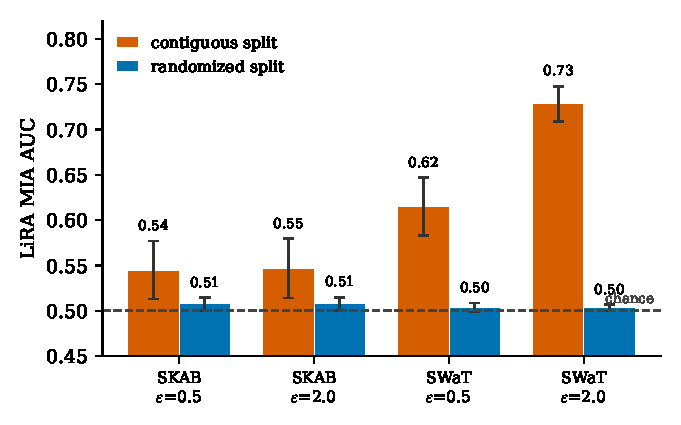
\includegraphics[width=0.7\linewidth]{figs/fig_mia}
\caption{Membership inference (LiRA AUC, mean$\pm$std over $5$ seeds). The contiguous member/non-member split (orange) produces apparent leakage---up to $0.73$
on SWaT---that collapses to chance once the split is randomized (blue). The artifact
is largest where the process drifts most (SWaT). Solid line marks chance. Bar labels
show means rounded to two decimal places (Table~\ref{tab:mia} reports three). Source:
\texttt{mia\_artifact.json}, \texttt{lira\_mia.json}.}\label{fig:mia}
\end{figure}

\subsection{Computational cost}\label{sec:res-runtime}
For completeness we report per-client cost (\texttt{runtime\_benchmark.json}). The
selection step is a one-time, cached cost of $0.6$--$1.7$\,s; the $3\sigma$ gate is
negligible ($<3$\,ms); a DP-SGD round costs $0.05$--$1.6$\,s; peak selection memory
is $6$--$32$\,MB. Per-round communication is identical with or without
deduplication (the model size is unchanged), so any benefit would have to come from
utility, not bandwidth---and we find none.

\section{Discussion and Limitations}\label{sec:discussion}

\paragraph{Scope: detection utility, not storage or integrity.} Our claim is
narrow and specific: data selection (deduplication, coresets) does not improve the
\emph{privacy--utility tradeoff of anomaly detection} under DP. It says nothing
about the other, legitimate reasons to deduplicate industrial data---storage and
bandwidth savings, retention-policy compliance, or fault-pattern preservation for
archival and audit. Those value propositions are orthogonal to detection utility
and are unaffected by our findings; a system can be worth deploying for storage
economy while offering no DP-utility benefit. We make this distinction explicit to
avoid over-reading ``deduplication does not help.''

\paragraph{Role of the suppression theorem.} It is worth being precise about
the role of~\cite{stoddard2026suppress}, because it explains one of our findings but not
the other. When selection statistics are computed on \emph{private} data---the uncontrolled pipeline---the selection map adds sensitivity that, at equal privacy, cancels the noise
saved by training on fewer samples; this is the suppression theorem, and it is exactly
why the uncontrolled utility gain is an artifact. But the leakage-controlled protocol computes selection
statistics on \emph{public} data, so $\varepsilon_{\text{sel}}=0$ and that
sensitivity-multiplication mechanism does not apply. The controlled-evaluation null---that no rule beats random or full even when selection is ``free''---is therefore an \emph{empirical}
finding, consistent with random subsampling being a strong baseline in the
high-compression regime~\cite{ayle2023bagging} rather than derived from the theorem. We
keep the two separate: the theorem accounts for the uncontrolled pipeline; the controlled null stands
on its measurements, which our longer-training experiment (\S\ref{sec:res-strong}) shows
are not an artifact of a detector stuck at the floor.

\paragraph{Limitations.} Our experiments use a reconstruction detector; other detector
families may differ in absolute F1, and we could not reach a point-wise high-signal
regime ($>0.6$) on these testbeds (\S\ref{sec:res-strong}). The empirical base is
effectively two ICS datasets: TEP saturates at its percentile threshold and serves
only as a $\rho\approx1$ control. Our membership-inference attacks use non-private
reference models and capped data, so a near-chance AUC bounds leakage \emph{under
these attacks} rather than proving its absence against an unbounded adversary; the
correct reading is ``no leakage detectable here'', not ``provably none''. The federated
study spans $K\in\{5,10,20\}$ contiguous clients ($R{=}15$ rounds) and the null holds
throughout (\S\ref{sec:res-selection}); still larger or more heterogeneous fleets
change the aggregation dynamics, and we do not claim the result transfers unchanged to
$K$ in the hundreds. The protocol also assumes a \emph{public} normal-operation
reference set for computing selection statistics; this is realistic for most ICS
deployments (a commissioning or maintenance period in known-normal operation) but not
universal, and where no such set exists the selection consumes privacy budget
($\varepsilon_{\text{sel}}>0$, composed with training as in~\cite{nguyen2025coreset})
and the public-data-absent setting is an open extension. We also state the scope explicitly: our findings concern reconstruction-based anomaly detection under
\emph{record-level} DP in ICS settings with $K\le20$ clients, and we do not claim they
transfer automatically to language or vision models, or to client-level DP. These bound
the scope of the claims; the protocol and the two artifact demonstrations do not depend
on closing them. The most consequential open direction is
whether the null survives a high-capacity sequential detector (e.g.\ a Transformer or
USAD-style model) that reaches genuine point-wise signal on these streams---the regime
our autoencoder cannot reach---together with a \emph{DP-aware} selection rule that
budgets its own sensitivity rather than spending none.

\section{Conclusion}\label{sec:conclusion}
Reliable measurement is the scarce resource in private IIoT learning. We gave a
leakage-controlled evaluation protocol for data selection under DP and used it to characterize two failure modes that a careless evaluation could mistake for results. The utility failure mode: a pipeline fits the selection gate on private data and trains the detector on a contaminated set, producing a large deduplication gain; under the protocol it
vanishes, and no rule we tried helps. The privacy failure mode: a membership-inference test that splits the stream by time reports apparent leakage (AUC up to $0.73$), but this
is process drift masquerading as membership; under a randomized, seeded split the
signal is chance, so the conclusion is that no leakage is detectable here. The unifying lesson is that in a DP pipeline both the training data and the evaluation
design are part of the privacy mechanism. Fit a selection rule on private data and you have spent
budget you did not record; let anomalies into a normal-only detector and you have
changed what it learns; split a drifting stream by time to test membership and you
will measure the drift, not the leakage.

This leaves a constructive open problem. The suppression
result~\cite{stoddard2026suppress} weighs against selection that ignores its own
privacy cost; it does not rule out \emph{DP-aware} selection that explicitly
budgets the sensitivity it introduces and spends $\varepsilon_{\text{sel}}$ against a
measured utility gain. Whether such a mechanism can beat random subsampling, and
whether selection helps for detector families with stronger point-wise signal on
these streams, are the questions our null makes precise.

\backmatter
\bmhead{Supplementary information} The full selection-comparison table (all budgets,
with standard deviations), the corrected-fit artifact-audit table, membership-inference
details and caveats, per-client runtime, and dataset/labelling details are in the
supplementary material.

\section*{Declarations}
\begin{itemize}
  \item \textbf{Funding.} Manipal University Jaipur.
  \item \textbf{Competing interests.} The authors declare that they have no known
    competing financial interests or personal relationships that could have appeared
    to influence the work reported in this paper.
  \item \textbf{Ethics approval and consent to participate.} Not applicable
    (no human or animal subjects; all datasets are public or testbed ICS data).
  \item \textbf{Consent for publication.} Not applicable.
  \item \textbf{Data availability.} The TEP benchmark is the publicly released
    Rieth et al.\ (2017) simulation campaign~\cite{rieth2017tep}, and SKAB is the
    official Skoltech release~\cite{katser2020skab}; both are openly downloadable.
    SWaT is the Mathur and Tippenhauer A4--A5 release~\cite{mathur2016swat,goh2016swat},
    obtained from iTrust (Singapore University of Technology and Design) under their
    usage agreement and therefore not redistributable by the authors. The
    SWaT attack-window labelling procedure is described in the supplement.
  \item \textbf{Materials availability.} Not applicable.
  \item \textbf{Code availability.} \textcolor{red}{[TODO before submission: archive the
    code repository at a frozen Zenodo DOI and insert the DOI here; do not state a link
    until it is live.]} The code and all result files
    needed to reproduce every reported number---including both the protocol-violating
    and the leakage-controlled pipelines---will be released at a permanent DOI upon
    publication.
  \item \textbf{Author contributions.} \textbf{R.S.~Gaur:} Conceptualization,
    Methodology, Software, Investigation, Writing -- original draft.
    \textbf{L.~Raja:} Supervision, Writing -- review and editing.
    \textbf{P.S.~Rathore:} Supervision, Methodology, Writing -- review and editing.
\end{itemize}

\bibliography{references}

\end{document}
